\section{Predictive evaluation}\label{sec:prediction}

A coefficient can describe the data well without improving forecasts. Two pre-registered
comparisons asked whether it does. Both refit every model at every origin, on data strictly
before the target.

\subsection{Designs}

\paragraph{Conditional prediction.} The first design predicts $\Delta u_{i,t}$ given all
data up to $t-1$ \emph{and} the GDP growth of quarter $t$, the setting the Okun equations
describe. There are two evaluation sets, each of \val{pc_quarters} target quarters:
2016--2019 (E1)
and 2022-Q3 to 2026-Q2 (E2). Five models are compared:
\begin{itemize}
  \item the hierarchical Bayesian model;
  \item its Gaussian i.i.d.\ variant;
  \item the OLS distributed lag;
  \item an ARDL model;
  \item a zero-change benchmark.
\end{itemize}

\paragraph{One-quarter-ahead forecasts.} The second design issues the forecast for quarter
$t$ at the end of $t-1$ and uses nothing dated $t$. There are \val{fc_origins} origins,
with targets from
2018-Q1 to 2026-Q2. It compares:
\begin{itemize}
  \item six classical models: persistence (a forecast of zero change), the historical mean, AR(1) of the change, two
    GDP lags, AR(1) with GDP lags, and that model with lagged participation;
  \item three hierarchical Bayesian forecasting models: an AR(1), AR(1) with GDP lags, and
    the same with a common factor.
\end{itemize}
The data are revised vintages, so the forecasts are retrospective, not real-time
(section~\ref{sec:data}).

\paragraph{Scoring.} Predictive distributions are scored with the continuous ranked
probability score (CRPS), a strictly proper scoring rule \citep{gneiting2007scoring}:
\[
  \mathrm{CRPS}(F,y)=\int_{-\infty}^{\infty}\big(F(z)-\mathbf 1\{z\ge y\}\big)^2\,dz .
\]
Scores are averaged over countries within each quarter, so that cross-country dependence is
handled at the level of quarters.

\paragraph{Inference.} The two designs use different procedures:
\begin{itemize}
  \item \emph{Conditional:} a Diebold--Mariano test on the quarterly mean differentials
    \citep{diebold1995accuracy}, with the small-sample correction of
    \citet{harvey1997dm};
  \item \emph{Forecasts:} a synchronised circular block bootstrap over target quarters.
\end{itemize}
Each family of pre-registered comparisons is Holm-adjusted.

\subsection{Results}

Each result below is the mean CRPS of the first model relative to the second; a negative
value favours the first.

\paragraph{Conditional prediction.} Decided comparisons: \val{pc_decided} of
\val{pc_total} (table~\ref{tab:predictive}, figure~\ref{fig:prediction}).
\begin{itemize}
  \item Before the pandemic, the hierarchical model against zero change: \val{pc_e1_zero}
    (Holm $p=$ \val{pc_e1_zero_holm}), the only decided comparison. It is fragile: in the
    registered sensitivity analysis without the target quarters in which a Bayesian refit
    failed, the Holm $p$ becomes \val{pc_e1_zero_holm_nofail}. The hierarchical model is
    practically equal to the classical regressions.
  \item After 2022, the hierarchical model against the OLS distributed lag:
    \val{pc_e2_ols} (Holm $p=$ \val{pc_e2_ols_holm}). No model that uses the quarter's GDP
    growth clearly beats zero change (hierarchical model against zero change:
    \val{pc_e2_zero}).
\end{itemize}

\paragraph{One-quarter-ahead forecasts.} Decided comparisons: \val{fc_decided} of
\val{fc_total}.
\begin{itemize}
  \item The hierarchical AR(1) with GDP lags against its classical counterpart:
    \val{fc_gdp} (95\% interval \val{fc_gdp_ci}). The gap comes mostly from
    2020-Q3 and 2020-Q4, where the classical GDP-lag regressions forecast badly; with so
    skewed a bootstrap distribution, the null-centred Holm-adjusted test does not decide it
    ($p=$ \val{fc_gdp_holm}).
  \item The hierarchical AR(1) with GDP lags against persistence: \val{fc_zero}.
  \item The hierarchical AR(1) against the classical AR(1): \val{fc_ar1}.
  \item Adding the common factor: \val{fc_factor}.
\end{itemize}
The protocol names one descriptive analysis in advance: the same comparisons without the
2020-Q1 to 2022-Q2 targets (\val{fcx_origins} target quarters). There, \val{fcx_decided}
of the five comparisons are decided in favour of the hierarchical or richer model
(Holm $p\le$ \val{fcx_holm_max}):
\begin{itemize}
  \item hierarchical AR(1) with GDP lags against the classical: \val{fcx_gdp};
  \item hierarchical AR(1) against the classical: \val{fcx_ar1};
  \item GDP lags within the hierarchical model: \val{fcx_lags};
  \item the common factor: \val{fcx_factor}.
\end{itemize}
The fifth comparison, the hierarchical model with GDP lags against persistence, also
favours the model on its point estimate (\val{fcx_zero}) but is not decided (Holm $p=$
\val{fcx_zero_holm}).

\paragraph{Reading the results.}
\begin{itemize}
  \item Over all target quarters the registered tests decide nothing; the pandemic
    targets dominate the loss differences.
  \item Outside the pandemic, partial pooling, lagged GDP growth and the common factor
    each improve the forecasts by a few per cent (\val{fcx_gain_lo} to
    \val{fcx_gain_hi}).
  \item No model reliably beats persistence, the forecast that the unemployment rate will
    not change. Persistence uses nothing but the last observed rate, and the classical
    AR(1) of the change does worse than it over all targets (\val{fc_ar1_vs_zero}).
  \item ``Not distinguishable'' never means ``equally accurate'': with
    \val{pc_quarters} or \val{fc_origins} target quarters, power is limited.
\end{itemize}

% Generated by eu-okun publication. Do not edit.
\begin{table}[t]\centering\small
\caption{Pre-registered predictive comparisons, mean CRPS of A relative to B (negative: A better). Conditional: GDP growth of the target quarter is known (panel Diebold--Mariano test). One-quarter-ahead: nothing dated $t$ is used (synchronised block bootstrap, 95\% interval). Holm adjustment within each family; a dash means not distinguishable at the 5\% familywise level.}
\label{tab:predictive}
\footnotesize\setlength{\tabcolsep}{4pt}
\begin{tabular}{lllrrl}
\toprule
Set & A & B & A vs B & Holm $p$ & Verdict \\
\midrule
Conditional E1 & Bayes primary & OLS distributed lag & $-0.5$\% & $1.000$ & --- \\
Conditional E1 & Bayes Gaussian i.i.d. & OLS distributed lag & $-1.2$\% & $1.000$ & --- \\
Conditional E1 & Bayes primary & Bayes Gaussian i.i.d. & $+0.7$\% & $1.000$ & --- \\
Conditional E1 & Bayes primary & ARDL & $-0.5$\% & $1.000$ & --- \\
Conditional E1 & Bayes primary & Zero change & $-13.5$\% & $0.018$ & A better \\
Conditional E2 & Bayes primary & OLS distributed lag & $-6.7$\% & $0.061$ & --- \\
Conditional E2 & Bayes Gaussian i.i.d. & OLS distributed lag & $-4.1$\% & $0.051$ & --- \\
Conditional E2 & Bayes primary & Bayes Gaussian i.i.d. & $-2.8$\% & $0.331$ & --- \\
Conditional E2 & Bayes primary & ARDL & $-8.5$\% & $0.131$ & --- \\
Conditional E2 & Bayes primary & Zero change & $-0.3$\% & $1.000$ & --- \\
\midrule
Forecast & Bayes AR(1)+GDP & AR(1)+GDP & $-15.3$\% $[-25.6, -2.9]$ & $0.276$ & --- \\
Forecast & Bayes AR(1) & AR(1) & $-1.4$\% $[-3.1, +0.5]$ & $0.276$ & --- \\
Forecast & Bayes AR(1)+GDP & Zero change & $+4.0$\% $[-6.8, +14.7]$ & $1.000$ & --- \\
Forecast & Bayes AR(1)+GDP & Bayes AR(1) & $+1.0$\% $[-3.3, +5.4]$ & $1.000$ & --- \\
Forecast & Bayes AR(1)+GDP+factor & Bayes AR(1)+GDP & $-5.5$\% $[-9.2, -1.9]$ & $0.230$ & --- \\
\bottomrule
\end{tabular}
\end{table}


\begin{figure}[t]\centering
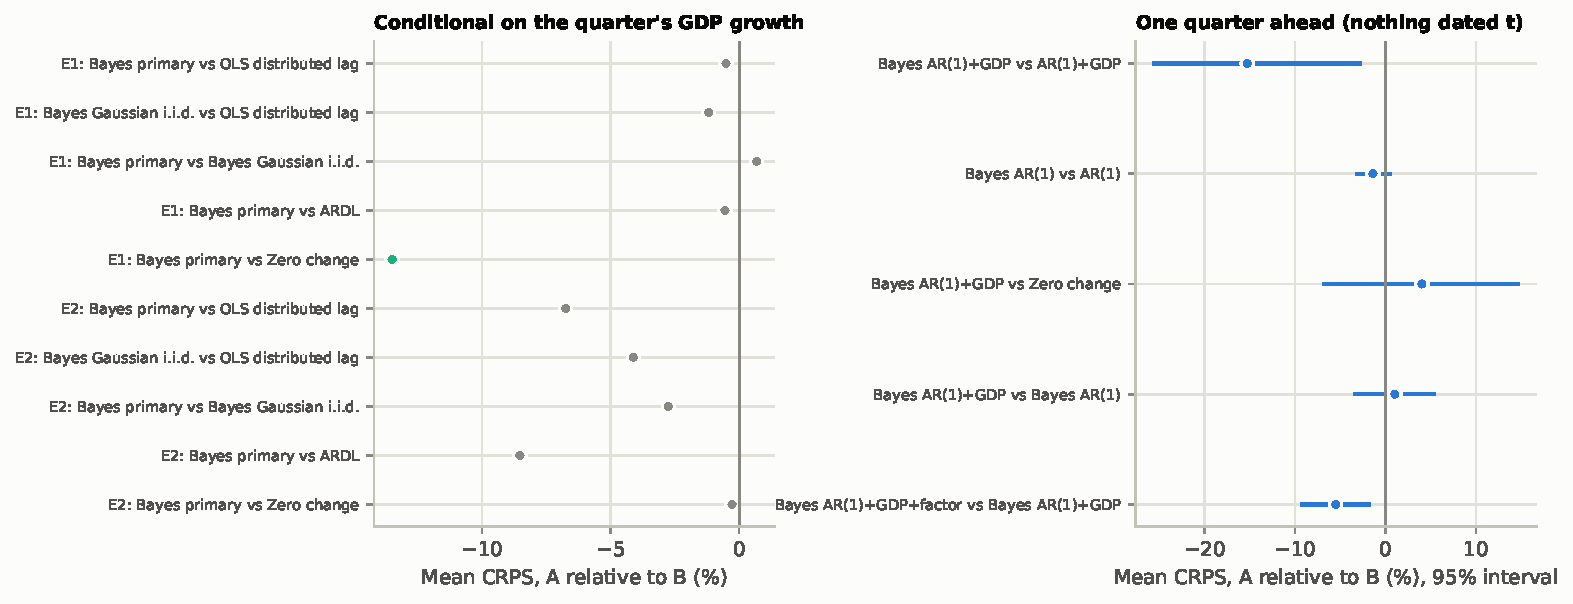
\includegraphics[width=\textwidth]{fig3_prediction.pdf}
\caption{Pre-registered predictive comparisons, mean CRPS of model A relative to model B
(negative: A better). Left: conditional on the quarter's GDP growth (green: decided at the
5\% familywise level). Right: one-quarter-ahead forecasts with 95\% bootstrap percentile
intervals. A percentile interval can exclude zero while the registered null-centred,
Holm-adjusted test does not reject, because two pandemic quarters skew the bootstrap
distribution.}\label{fig:prediction}
\end{figure}
